\subsection{Mock Data Providers}

Coordinating and managing real data providers while developing or testing can be challenging.
FLOps offers its own mock data providers to make these processes more convenient.
These optional services can be deployed on learner nodes via the orchestrator.
They split datasets into partitions and send them to the ML data server exactly as real devices.
It is enough to run them once to populate the local learner nodes with data.
These mock data providers also act as implementation examples for real devices when converting data, setting up a Flight client, and communicating with an ML data server.
The code is available here \cite{flops_code}.
Subsection \ref{subsection:api} shows the API endpoint for creating such mock data providers.
The FLOps Helper SLA for mock data providers looks as follows:
\begin{lstlisting}
    {   % The ID has to match the user's orchestrator ID.
        "customerID": "Admin",
        "mock_data_configuration": {
            % This value can be any dataset name available in Hugging Face.
            "dataset_name": "cifar10",
            "number_of_partitions": 1,
            "data_tag": "cifar10" 
        }
    }
\end{lstlisting}
\begin{figure}[h]
    \begin{adjustwidth}{-0.1\paperwidth}{-0.1\paperwidth}
        \centering
        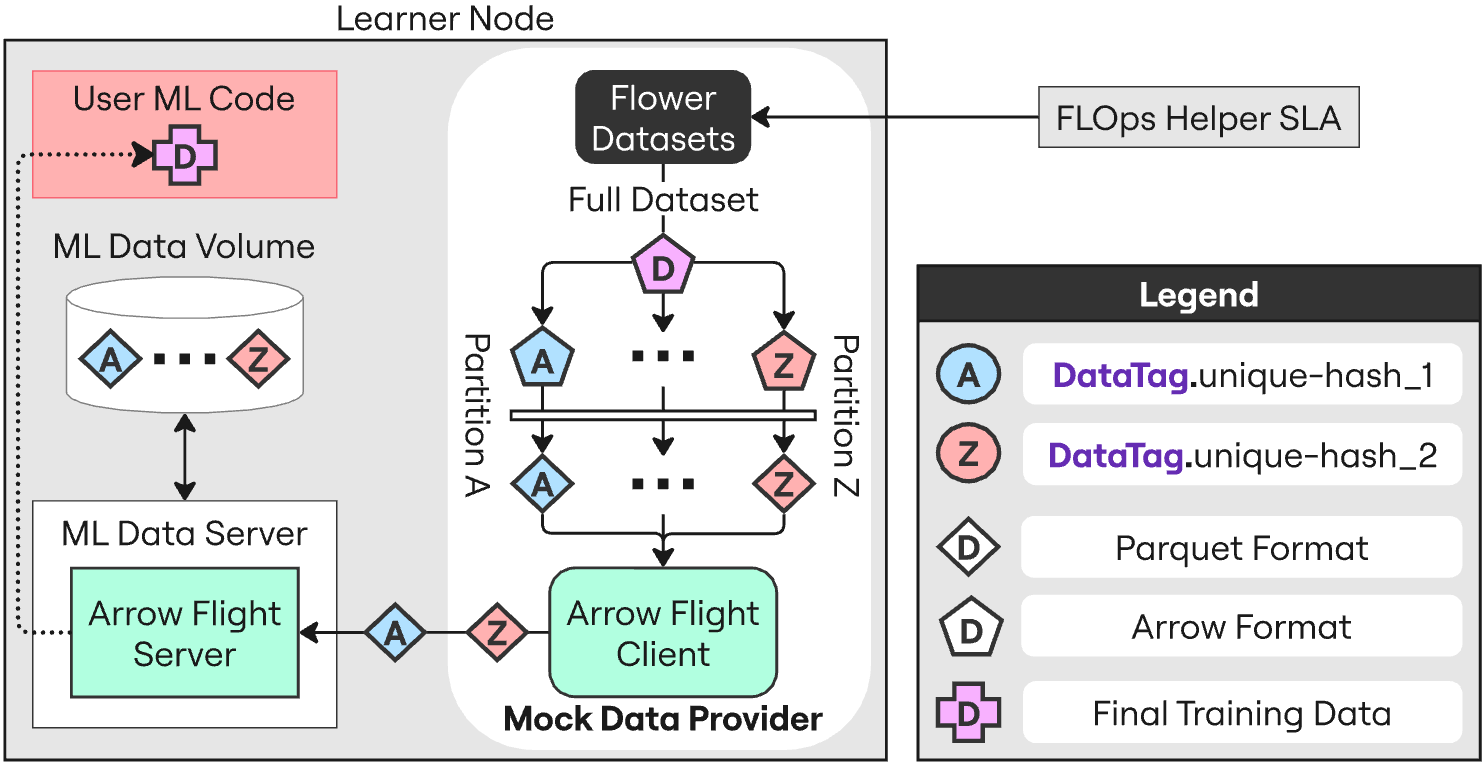
\includegraphics[width=0.80\paperwidth]{mock_data_provider.png}
        \caption{FLOps' Mock Data Provider}
        \label{fig:mock_data_provider}
    \end{adjustwidth}
\end{figure}
Figure \ref{fig:mock_data_provider} depicts FLOp's mock data provider.
The mock data provider runs as an orchestrated service in the container execution environment, similar to the learner service.
It uses the requested Hugging Face dataset name to download the dataset via Flower Datasets.
The data provider uses Flower Datasets to split this monolith dataset into multiple partitions.
The user defines the number of partitions.
Each partition is individually sent to the ML data server as if real edge devices were contacting the server.
The ML data server stores each partition separately in the ML data volume.
Ultimately, these partitions will be merged and preprocessed to be fit for training.
